\documentclass[conference]{IEEEtran}
%\usepackage{cite}
\usepackage[backend=biber,citestyle=ieee]{biblatex}
\usepackage[T1]{fontenc}
\usepackage[utf8]{inputenc}
\usepackage{amsmath, amssymb, amsfonts}
\usepackage{algorithmic}
\usepackage{graphicx}
\usepackage{textcomp}
\usepackage{xcolor}
\addbibresource{report.bib}

\graphicspath{{imgs}}
% What is this?
\def\BibTeX{{\rm B\kern-.05em{\sc i\kern-.025em b}\kern-.08em
    T\kern-.1667em\lower.7ex\hbox{E}\kern-.125emX}}


\begin{document}
\title{Data Science Final Project Report}
\author{\IEEEauthorblockN{Andr\'es Ponce}
		\IEEEauthorblockA{\textit{Department of Computer Science} \\
		\textit{National Cheng Kung University} \\
		Tainan, Taiwan \\
		andresponce@ismp.csie.ncku.edu.tw}
}
%\author{\IEEEauthorblockN{1\textsuperscript{st} Given Name Surname}
%\IEEEauthorblockA{\textit{dept.\ name of organization (of Aff.)} \\
%\emph{name of organization (of Aff.)}\\
%City, Country \\
%email address or ORCID}
%}

\maketitle
\begin{abstract}
	Many e-commerce platforms need to search for similar or identical products
	given some query image.
	Doing so can increase the platform's ability to recommend interesting 
	products or analyze purchasing trends across product categories.
	For the eBay eProduct Visual Search Challenge, participants take a set
	of query images and search a large index set for matching products.
	We first train a model to recognize the hierarchical structure of the different
	image categories.
	Then, we use our model's output to produce hashes of the index images
	and query images, and locate identical products by comparing these hashes.
	This paper describes our method, experiments, and results used in this
	competition.
\end{abstract}

\section{Introduction}
E-commerce platforms continue to grow and play a large role in consumer's
shopping behavior.
Especially with the pandemic, more people relied on such platforms for 
many of their purchases~\cite{jilkova2021digital}.

Platforms where users directly sell their own products especially
benefit from finding images of identical products.
When a user searches for a product, he or she expects the results to contain
images of the same product.
On sites like eBay, identifying identical products can be very useful when 
aggregating sales of different listings of the same product.
Not only do e-commerce platforms rely on such visual search, but also visual
search engines such as Google Images, where the user can use an image as a query
instead of a search term.

The eBay eProduct Visual Recognition Challenge~\cite{jiangbo2021ebay} consists of
finding images of the same product from a large index set of images.
This challenge is one of fine-grained visual classification, since we are trying to 
find images of \emph{the same} product. 
Similar products can differ by very small details, increasing the difficulty of the task.
Likewise, identical products might differ based on lighting conditions or other yet 
our model should still identify identical products despite these factors.

\section{Competition Description}
Current image datasets do not focus enough on super fine-grained object detection.
This prompted the authors to create the eProduct dataset focusing on fine-grained
visual recognition.
The dataset is divided into training, validation, and query sections. 

The training set consists of around 1.3 million labeled images modelled after the ImageNet~\cite{deng2009imagenet} dataset.
Each image also three levels of hierarchical labels: its meta class (16 total), level 2 class (17 total),
and the leaf class (1,000 total) as well as the product title and unique identifier.
Also similar to ImageNet, the validation set contains 50,000 images, each containing the same information 
as the training set.

The testing set contains 10,000 query images with only the unqiue identifier information.
Given one of these query image, our task is to search for matching products to this query in a 1.1 million image index set, also provided
as part of the testing set.
The index set contains \emph{groundtruth sets} which are a match with any of the query images and 
a \emph{distractor set} which does not match with any query image.

\begin{figure}[!t]
\centering
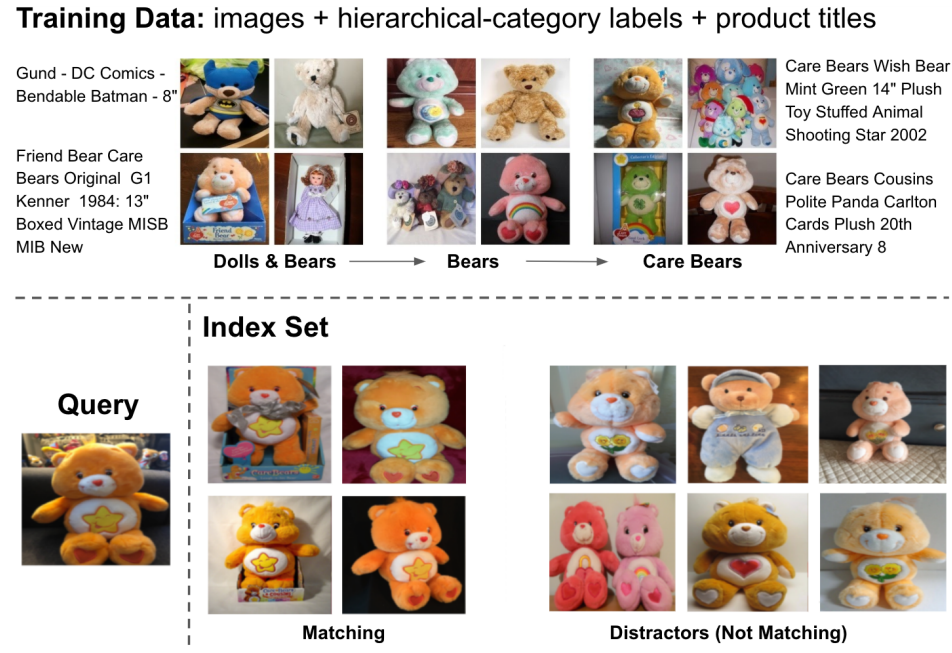
\includegraphics[scale=0.25]{structure}
\caption{eProduct dataset structure. The top section contains a sample training image and the meta,
level 2, and leaf categories. Each level contains a more specific type of product, and the leaf category
can still contain slightly different, non-matching products. 
The bottom section shows the query image and the identical products from the index set, along with a set 
of \emph{distractor} products that do not match with any query image.}

\label{fig:structure}
\end{figure}

\section{Method}
\section{Training and Experiments}
 \printbibliography
\end{document}
